\chapter{Natural Lifetime}

Every object created by your application lives for an interval of time from its
creation to the point that the Java runtime gets around to collecting it. For
some subset of an object's {\em actual} lifetime, your application will make use
of its fields. An object's {\em natural} lifetime is defined by the interval of
time between its first and last necessary use. %%%%% cite drag paper here?
It is important to appreciate this distinction, between natural and actual
lifetime, so that you can implement your code in a way that avoids bugs and
performs well in the case when not everything fits into the Java heap.

The Java runtime takes care of some of these issues, but leaves a great many in
your hands. In Java, you needn't explicitly free objects, and in that way a
managed language is a big step up from a language like C. However, the the
promise of automatic memory management, that it frees you from the burden of
managing memory, doesn't play out as well in practice. When programming in Java
it is important to think through whether your application needs an object to live
forever, or, if not, when you expect it to die. With these thoughts in mind, you
can plan how to  implement the right lifetime policies. You have to be careful
to do so without introducing memory leaks or performance problems. This entails
combining the tools that Java  provides with other strategies, implemented on
top of Java.


\section{Planning out Object Lifetime}

\begin{figure}
	\centering
	\subfigure[The lifecycle of a typical object and its data.]{
		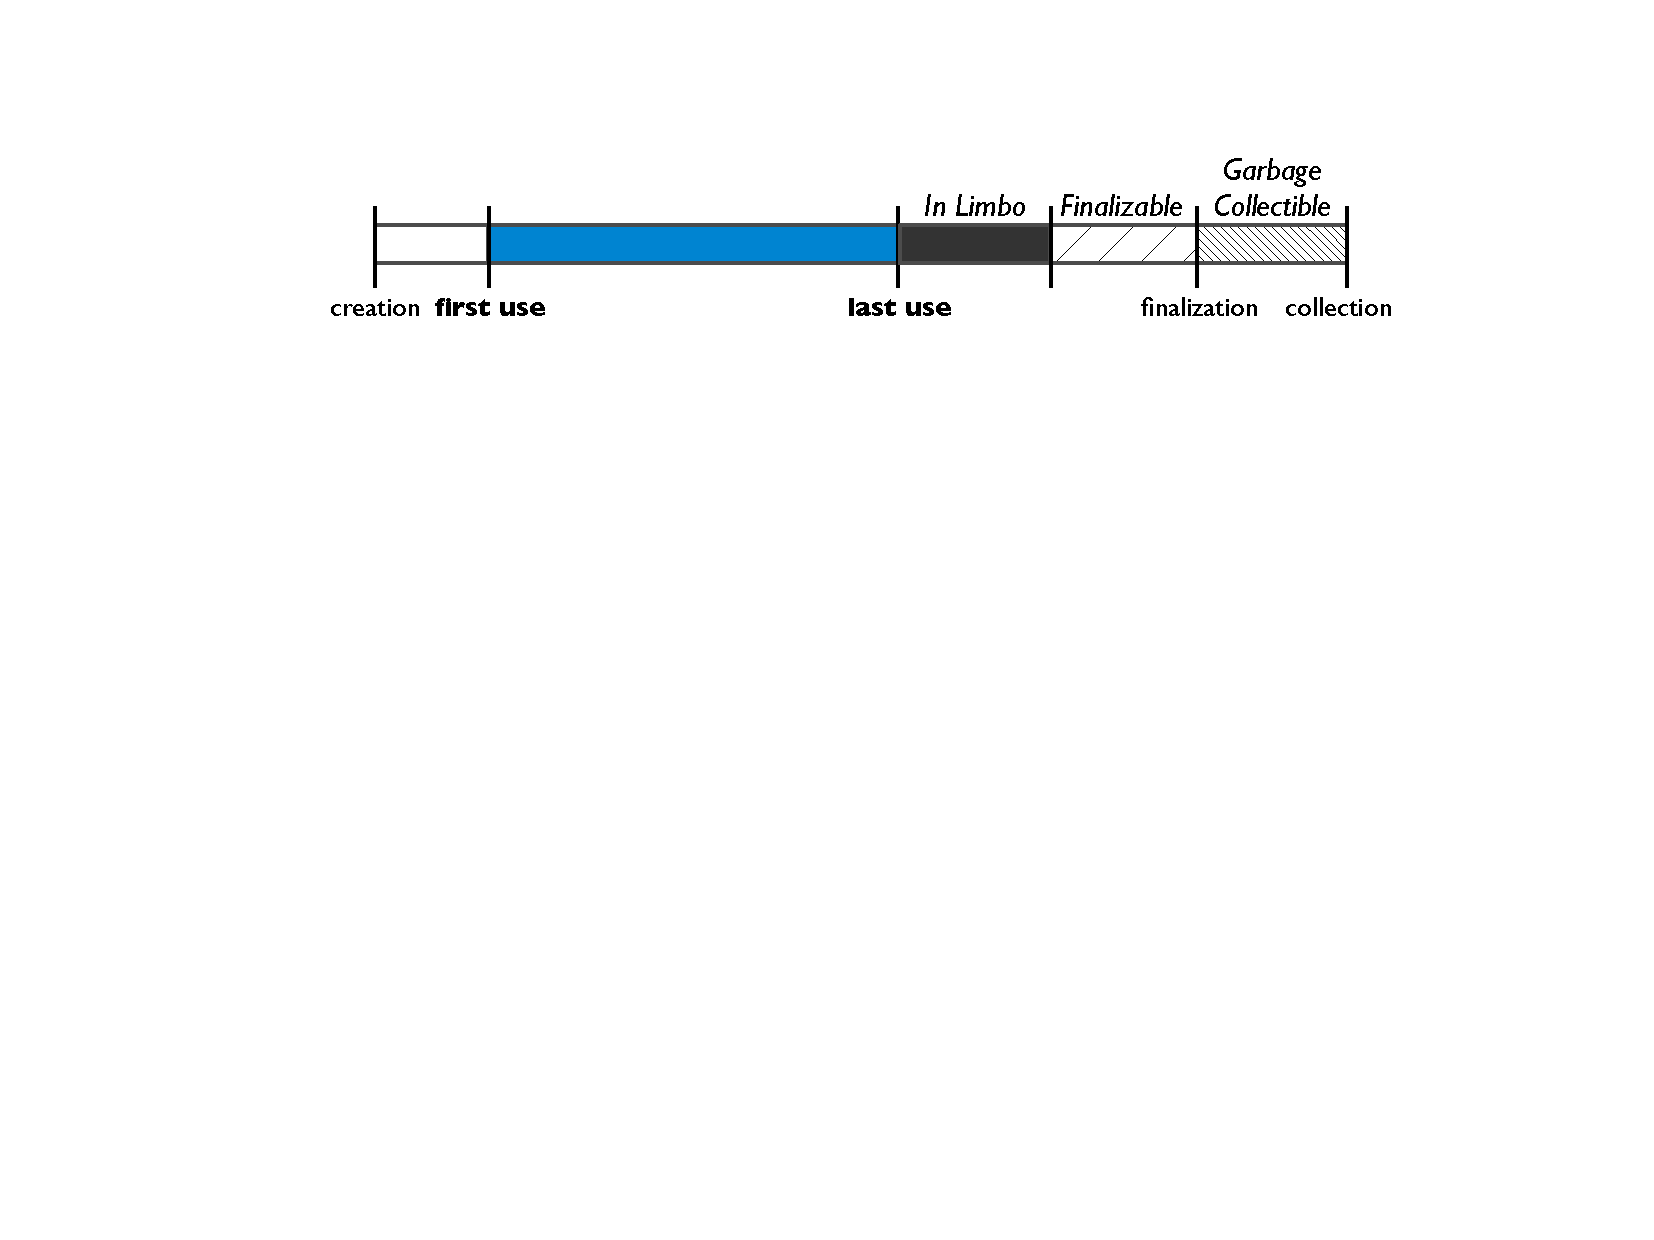
\includegraphics[width=0.8\textwidth]{Figures/object-lifecycle}
	}
	\subfigure[The lifecycle of the data  that is loaded from
	disk three times, and the objects that store it.]{
		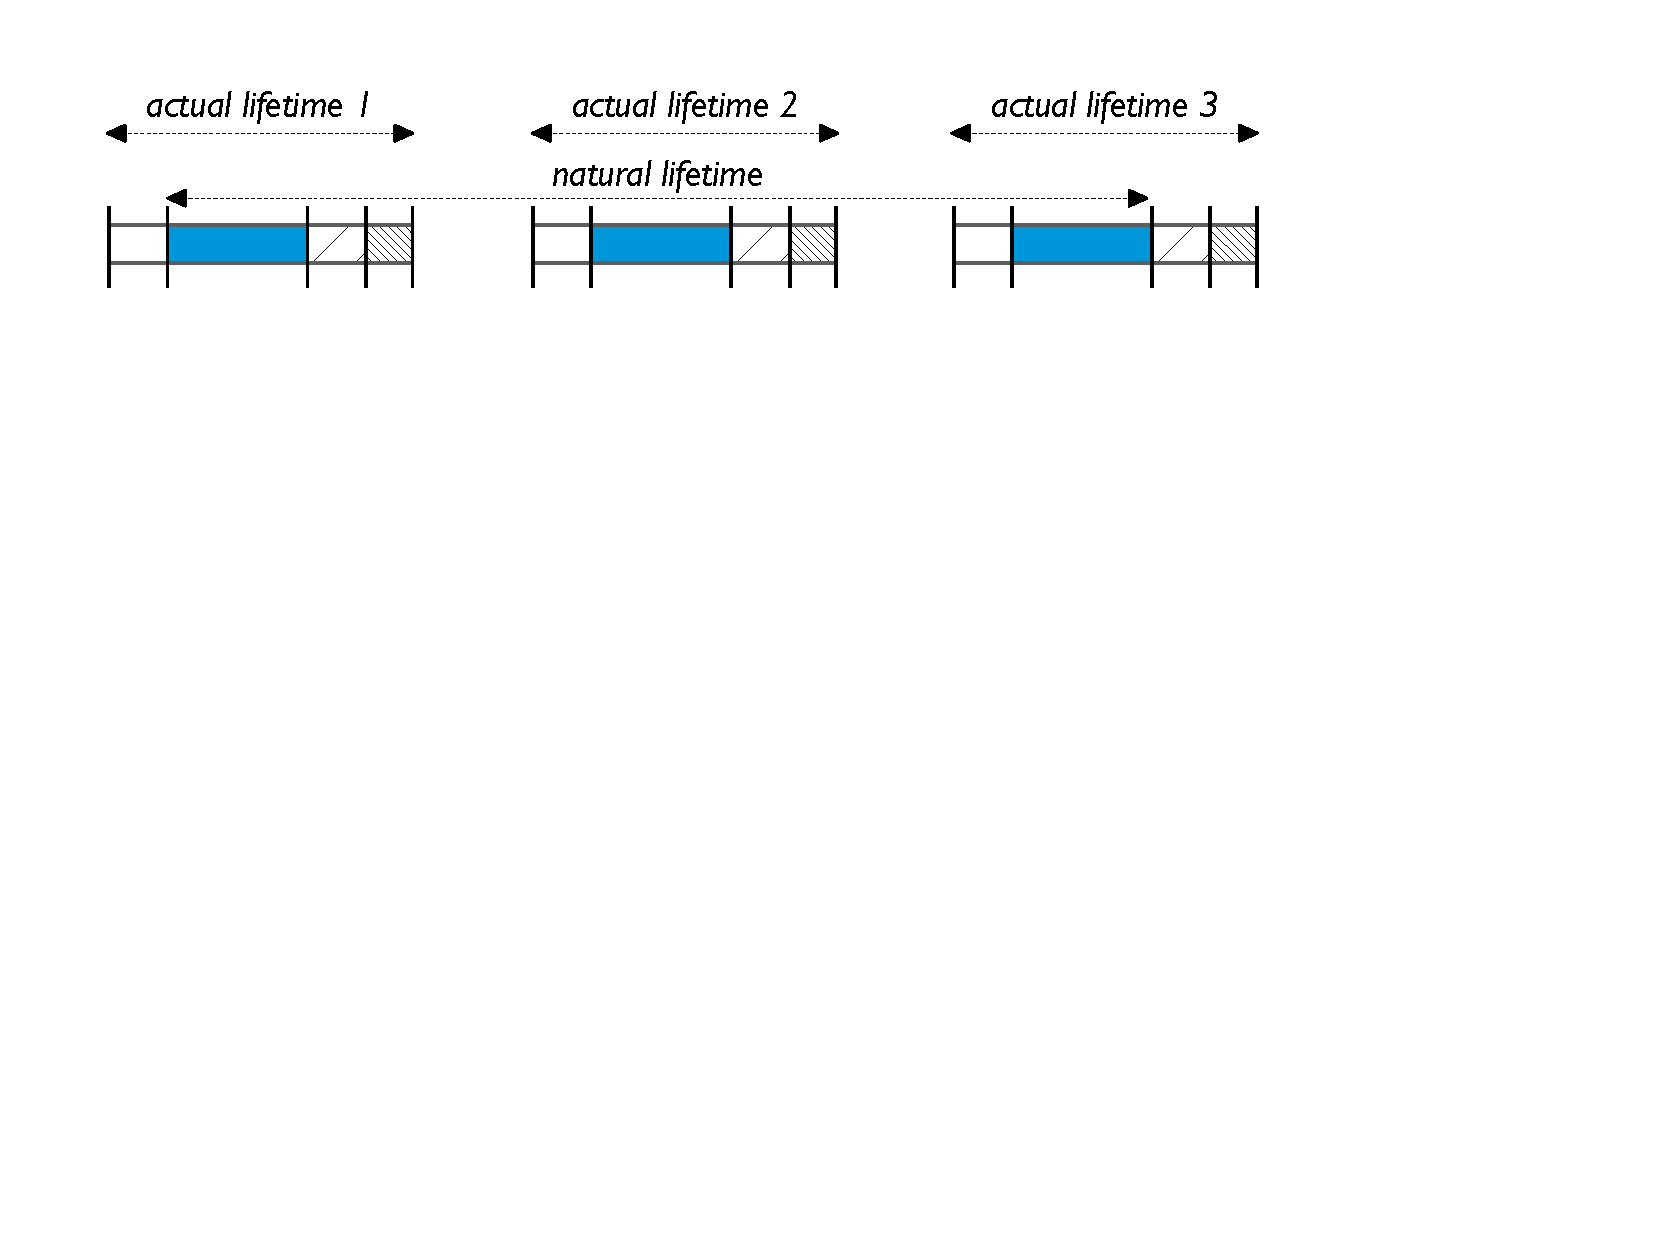
\includegraphics[width=0.8\textwidth]{Figures/object-lifecycle2}
	}
	\caption{Examples of Natural and Actual lifetimes.}
	\label{fig:typical-lifecycle}
\end{figure}


\begin{table}
\centering
\begin{tabular}{|l|l|} \hline
long-lived & needed forever \\ \hline 
correlated lifetime & \shortstack{needed for a period\\ 
scoped to a phase/request\\
correlated with an object (annotations)\\
correlated with need}\\ \hline
reusable & maybe i'll need it later \\ \hline
\end{tabular}
\end{table}

% correlated with need: as soon as last user goes away, remove his stuff 
% share common expressions to save space, but using strong references -> memory
% leak; plugins in eclipse go away when all views
% sharing pool 

% weak ref keys -> annotation
% weak ref values -> sharing pool

% soft ref values -> caching

% annotation by map lookup


\section{Objects Needed Forever}

Created and used for the remaining duration of a run.


\section{Correlated Lifetime}

Many objects are created and then only needed for some interval of time. For
example, say your application is a transaction processing system implemented as
a Java Enterprise Edition web application. In this case, most objects
created within the scope of a servlet request will not, and for correctness
reasons {\em must not}, survive the request; they are not used by the 
application after the request has completed, and will, in the absence of bugs,
be collected as soon as is convenient for the runtime. In this example, the
lifetime of objects during a request are {\em correlated} with a method
invocation: when the servlet \class{doGet} or \class{doPut} (etc.) invocations
return, those correlated objects had better be garbage collectible.

The same is true for a great many objects created by the application, not just
at the large granularity of a servlets. For example,

In many cases, the built-in mechanisms 

\section{Delayed-Deletion}

A cache is a performance optimization that holds on to a data structure after the
current operation is finished with it, in the hope that other operations in the
near future will reuse it. The expense of re-fetching data from external data
sources and recomputing the in-memory structure can often be amortized, at the
expense of stretching the lifetime of these data structures. By increasing the
actual lifetime on an object you will very likely increase peak memory
consumption.




%if scopes don't coincide with lifetime

\begin{table}
\centering
\begin{tabular}{|l|l|} \hline
\em mechanism & \\ \hline \hline
stack & \\ \hline 
static & \\ \hline
thread-local & \\ \hline
soft & \\ \hline
weak & \\ \hline
phantom/finalizers & \\ \hline
memory mapping & via \texttt{java.nio} \\ \hline 
object serialization & \\ \hline
\end{tabular}
\caption{Built-in lifetime management mechanisms.}
\label{tab:builtin-lifetime-management}
\end{table}

\begin{table}
\centering
\begin{tabular}{|l|l|} \hline
\em mechanism & \\ \hline \hline
resource pool & \\ \hline
cache & \\ \hline
sharing pool & (interning)\\ \hline
memoization & \\ \hline
backing store &(externalized memo) \\ \hline
non-OO & (column orientation) \\ \hline 
\end{tabular}
\caption{Lifetime management mechanisms not provided by the Java language that one must implement.}
\label{tab:software-lifetime-management}
\end{table}




%% OLD STUFF NMM 20090820
%\section{Request Scoping}
%\section{Correlated Lifetime}
%\paragraph{Weak and Soft references in Java}
%\section{Memory Leaks and Drag}
%\section{Examples}
%\subsection{Transient Near-Copies}
%\subsubsection{String Canonicalization}
%\subsection{Temporary Collections}
%\subsection{Facilitators}
